\documentclass[12pt]{article}
\usepackage[utf8x]{inputenc}
\usepackage{amsmath}
\usepackage{multicol}
\usepackage{graphicx}
\usepackage{float}
\usepackage{dsfont}
\usepackage{textcomp}
\usepackage{amsfonts}
\usepackage{cleveref}
\usepackage[T1]{fontenc}
\usepackage[colorinlistoftodos]{todonotes}
\usepackage[margin=2.5cm,a4paper]{geometry}
\usepackage{listings}
\setlength{\marginparwidth}{2cm}
\setlength{\parindent}{0pt}
\newcommand{\deriv}{\mathrm{d}}
\lstset{
    language=R,
    basicstyle=\scriptsize\ttfamily,
    commentstyle=\ttfamily\color{red},
    numbers=left,
    numberstyle=\ttfamily\color{blue}\footnotesize,
    stepnumber=1,
    numbersep=5pt,
    backgroundcolor=\color{white},
    showspaces=false,
    showstringspaces=false,
    showtabs=false,
    frame=single,
    tabsize=2,
    captionpos=b,
    breaklines=true,
    breakatwhitespace=false,
    title=\lstname,
    escapeinside={},
    keywordstyle={},
    morekeywords={}
    }
\title{}
\begin{document}
\begin{titlepage}
\newgeometry{left=1.5in,right=1.5in,top=2.5in,bottom=2.5in}
\newcommand{\HRule}{\rule{\linewidth}{0.5mm}}
\begin{centering} 
%---------------------------------------------------------------------------
%	HEADING SECTIONS
%---------------------------------------------------------------------------

\includegraphics[scale=0.6]{Images/Uni_of_Kent.png}\\[1cm]
%---------------------------------------------------------------------------
%	TITLE SECTION
%---------------------------------------------------------------------------
\HRule \\[0.4cm]
\textsc{\large Astronomy, Space Science and Astrophysics}\\[0.5cm]
{ \Huge \bfseries Biot-Savart's Law}\\[0.4cm]
\HRule \\[1.0cm]
%---------------------------------------------------------------------------
%	DATE SECTION
%---------------------------------------------------------------------------
\textsc{\Large PH520 - Stage 2}\\[0.4cm] 
\textsc{\Large Physics Laboratory A}\\[0.4cm] 
{\large Date: 30th Sept - 21st Oct 2019}\\[0.4cm]
%---------------------------------------------------------------------------
%	AUTHOR SECTION
%---------------------------------------------------------------------------
\begin{minipage}{0.625\textwidth}
\begin{center} \large
\emph{Report Author:} Lukasz R Tomaszewski \\[0.2cm]
\emph{Lab Partner:} Stephanie Wood \\ [0.5cm]
{\large Word Count: 2716}\\
\end{center}
\end{minipage}\\[2cm]
\vfill
\end{centering} 
\end{titlepage}
%---------------------------------------------------------------------------
%	CONTENTS   -------------------------------------------------------------
%---------------------------------------------------------------------------
\newpage
\begin{titlepage}
\begin{tableofcontents}
\end{tableofcontents}
\end{titlepage}
\newpage
%\begin{multicols}{2}
%---------------------------------------------------------------------------
%	ABSTRACT
%---------------------------------------------------------------------------
\section{Abstract}

This experiment proves the mathematical equations are flawed in a sense of being perfect, a physical simulation shows that many external factors effects the magnetic field not only those factors that were intended to change. To talk about about change, the magnetic field was theoretically proven to change, showing in a physical simulation; current, distance, angle and different types of conductors shapes and sizes directly affect the magnetic fields shape, size and strength. Though operating within expected error; $\pm$0.005mT, $\pm$0.005m/0.001m , $\pm$5\textdegree, it was shown that many external environmental factors alter a physical replication of the theoretical data.

%---------------------------------------------------------------------------
%	INTRODUCTION
%---------------------------------------------------------------------------
\section{Introduction}

"Due to the technological advancements of the human race, from electric power to computer storage, magnetic fields have been heavily exploited. Even though magnetic fields occur when charges or currents are moving, they tend to be very weak. Amperes law and Biot-Savarts law help calculate a magnetic field due to the a particular arrangement of current. Within this experiment all measurements rely on an axial B-probe, this records the strength of the magnetic field in the direction of the probes axis, thus the probes orientation must be carefully aligned with the apparatus. Keeping the probe in a fixed position is key as background magnetic fields can interfere and move the artificial magnetic field instead of the probe itself." \cite{Exp.5-2019}\cite{Exp.5-Lab_book}. \\

This experiment will help deduce the two questions (\cref{Data Collected}) and provide insight on how magnetic fields are affected by different conductors, current and distance while observing any and all external factors. This can be assessed by calculating the theoretical results and comparing them with actual results obtained in a practical simulation.

%---------------------------------------------------------------------------
%	METHODOLOGY
%---------------------------------------------------------------------------
\section{Methodology}
\subsection{Apparatus}
\begin{multicols}{2}
\begin{itemize}
	\item Connection cables
	\item Axial B-probe
    \item Teslameter
    \item Assorted conductors
    \item Air solenoid stand
    \item Conductor holders
	\item Air solenoid (variable lengths)
    \item Pair of Helmholtz coils
    \item High current power supply
    \item Stand base with small optics bench
\end{itemize}
\end{multicols}

\subsection{Data collected}
\label{Data Collected}
The data collected shall be the magnetic field (measured by the Axial B-probe) due to various current carrying conductors, i.e the magnetic field of:
\begin{multicols}{2}
\begin{itemize}
    \item An air solenoid
    \item An straight conductor
    \item 40mm, 80mm and 120mm diameter conductor loop
    \item A single and pair of Helmholtz coils
\end{itemize}
\end{multicols} 

\underline{Questions}:
\begin{itemize}
    \item "What is the direction and strength of the Earth's magnetic field in the physics laboratory?" \cite{Exp.5-2019}
    \item "If the pair of Helmholtz coils were wired in the other direct (one clockwise, the other anti-clockwise), what would the magnetic field be like between the Helmholtz coils?" \cite{Exp.5-2019}
\end{itemize}

\subsection{Risk assessment}

"Within this experiment there are two hazards that pose serious concerns; electroshock, burns and electrocution from the apparatus (connected to the mains) used and the danger of bruising and severe injury from dropping the heavy apparatus/ appliances. Ensuring that all electrical appliances have a valid PAT (portable appliance test) sticker and keeping all of the apparatus away from the edge of the table will ensure a lower risk factor. Furthering the safety of this experiment regarding the operational use of the appliances, although the currents are maxed at 16 Amps, it shouldn't cause any serious harm if electrocuted. As the conductors/ cables will be carrying a continuous stream of current, the conductors/ cables will get hot after an extended time so great care must be taken when handling the apparatus." \cite{Exp.5-2019}\cite{Exp.5-Risk}\cite{Exp.5-Lab_book}

\subsection{Useful constants}
\label{constants}

\begin{table}[H]
\begin{center}
 \begin{math}
 \begin{tabular}{c c c}
 Permeability of free space & $u_0$ & $4\pi x10^{-7}Hm^{-1}$ \\
 Number of turns in Air Solenoid & $N_{Air}$ & 30 Turns \\
 Radius of Air Solenoid & $R_{Air}$ & 4.2cm (0.042m) \\
 Number of turns Helmholtz Coil & $N_{HC}$ & 320 Turns \\
 Radius of Helmholtz Coil & $R_{HC}$ & 6.75cm (0.0675m) \\
 \end{tabular}
 \end{math}
 \caption{Useful Constants \cite{Exp.5-2019}}
 \label{Useful Constants}
\end{center}
\end{table}

\subsection{Error analysis}

\begin{table}[H]
\begin{center}
 \begin{math}
 \begin{tabular}{c c c}
 Teslameter = & $\pm$0.005mT \\
 Rounding Error = & $\pm$0.05mT, $\pm$0.005m \\
 Total Error = & $\sqrt{(0.005)^2 + (0.005)^2}$ = & $\pm$0.007mT\\ [0.5cm]
 
 Angle Error = & $\pm$5\textdegree \\
 'r' distance = & $\pm$0.001m \\
  Total Error = & $\sqrt{(5)^2 + (0.001)^2}$ = & $\pm$5\textdegree\\
 \end{tabular}
 \end{math}
 \caption{Error Analysis \cite{Exp.5-Lab_book}}
 \label{Error Analysis}
\end{center}
\end{table}

\subsection{Experimental procedures}

\subsubsection{Magnetic field due to conductors}

Starting with the set up stated in \cref{CL setup} below, placing the axial B-probe into the centre of the 40mm conductor loop with the current turned off, adjusting the axial B-probe position to find the highest value on the teslameter, setting the teslameter to zero before turning on the current allows for accurate readings without any residual background interference. Keeping the axial B-probe stationary and adjusting the current shows that the magnetic field is directly related to current. \\

\begin{figure}[H]
\centering
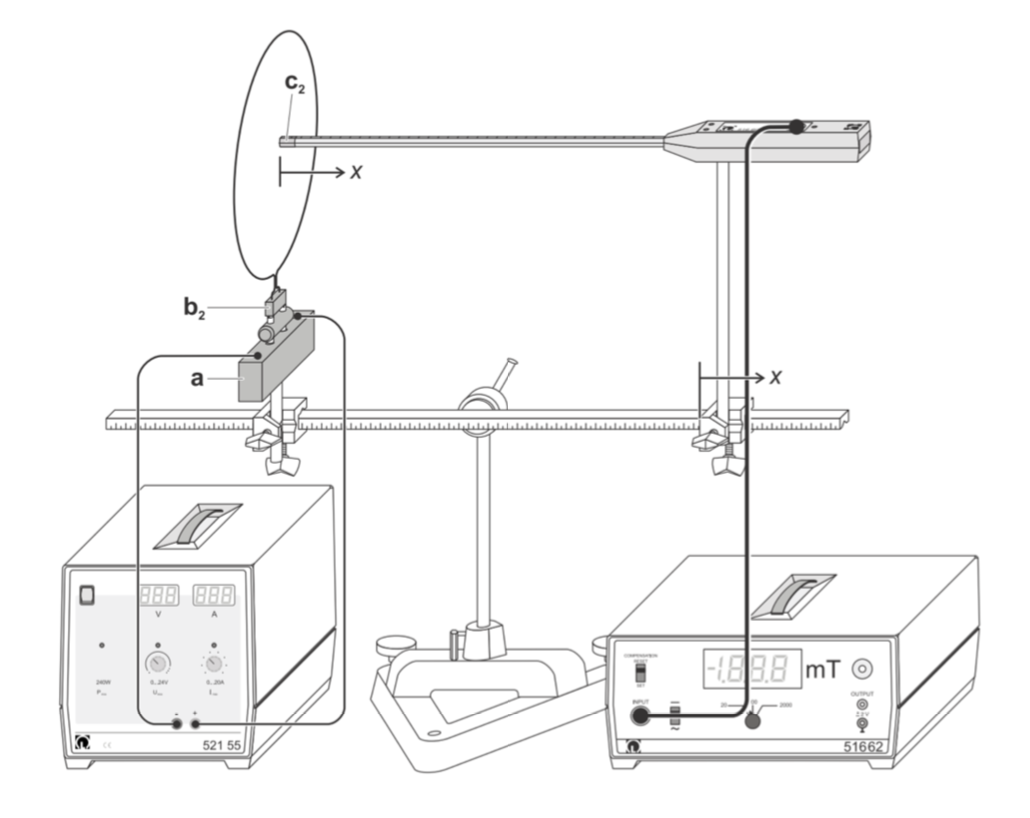
\includegraphics[scale=0.4]{Images/CL.png}
\caption{Conductor loop setup. \cite{Exp.5-2019}}
\label{CL setup}
\end{figure}

By keeping the current steady at 16 Amps, a relationship between the magnetic field and distance of the axial B-probe is formed as moving loop 10cm in 1cm increments in both directions grants insight on how the magnetic field behaves. By repeating this but with larger diameter conductor loops and a new relationship is formed. Utilizing a 80mm and 120mm diameter conductor loop, ensuring they are centred and zeroed before readings were taken. \\

\begin{figure}[H]
\centering
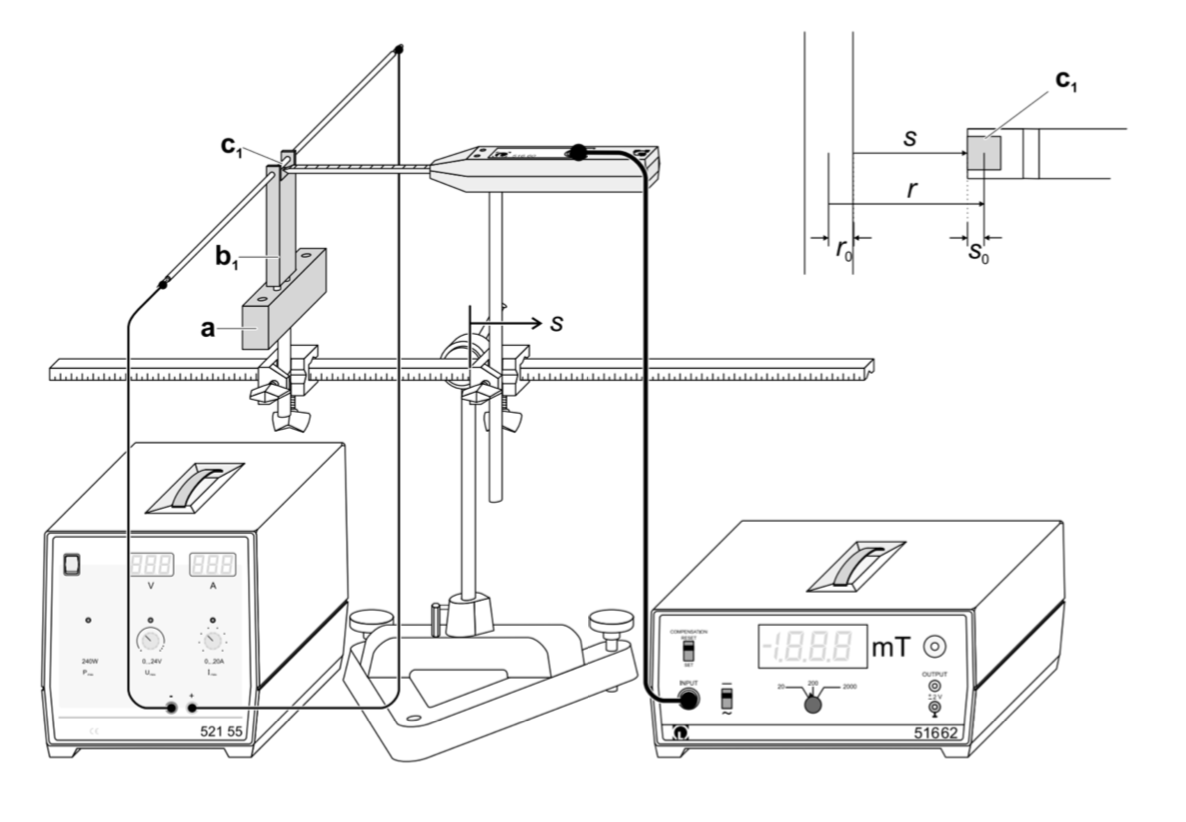
\includegraphics[scale=0.4]{Images/SC.png}
\caption{Straight conductor setup. \cite{Exp.5-2019}}
\label{SC setup}
\end{figure}

A loop creates a specific shape of magnetic field, a long wire creates another shape, keeping the current at 16 Amps, and measuring axially from an zeroed offset provided in \cref{SC setup}. Moving the loop 3cm in 0.5cm increments in both directions provides the proof of the change of shape the magnetic field has undertaken from that of the conductor loops.

\subsubsection{Axial magnetic field of an air solenoid}

Changing to the air solenoid conductor stated below in \cref{AS setup}, again centering and zeroing the axial B-probe in a fixed position to obtain accurate readings. Firstly to see how the current affects the magnetic field, keeping the coil length at 15cm and adjusting the current up by 2Amps to 16 Amps. A new relationship is formed and thus can be also compared to distance as changing the length of the coil from 10cm to 40cm in 5cm increments while keeping a steady current at 16Amps gives the distance-magnetic field relationship.

\begin{figure}[H]
\centering
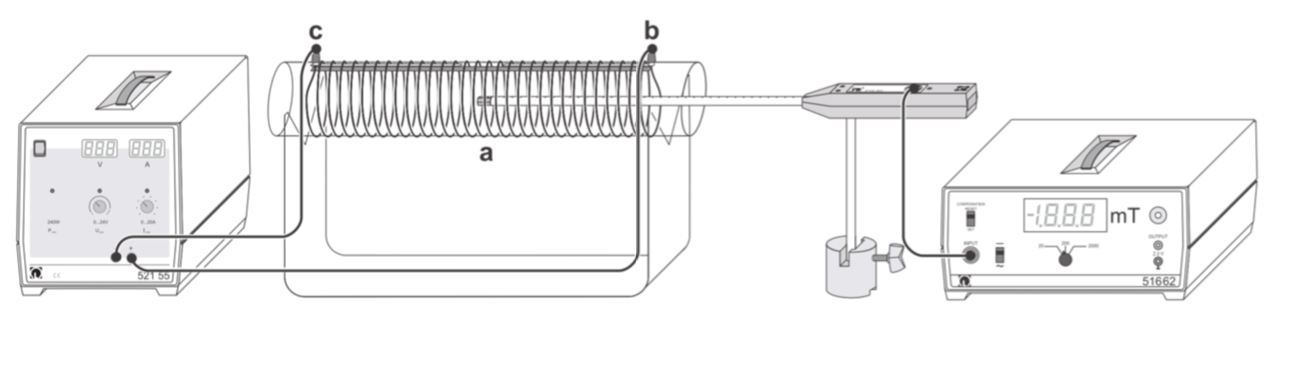
\includegraphics[scale=0.5]{Images/AS.png}
\caption{Air solenoid conductor setup. \cite{Exp.5-2019}}
\label{AS setup}
\end{figure}

Furthering the relationship between distance and the magnetic field, adjusting the length of the coil in 2cm increments 20cm in either direction allows further insight onto this relationship. The axial B-probe will need to be moved and placed in the opposite direction due to the limitations of length that the apparatus provides, ensuring that the probe is zeroed for accurate readings.

\subsubsection{Radial and tangential magnetic field of an Helmholtz coil}

So far a relationship between current/ distance and the magnetic field have been established, furthering the insight of how magnetic fields behave with angles, a single Helmholtz coil is used. Beginning with a same setup in \cref{CL setup} but changing the conductor loop with the Helmholtz coil, setting the axial B-probe on an offset on the same axis so the teslameter reads 0.15mT to allows complete rotation of the coil. Turning the Helmholtz coil a full rotation, reading the magnetic field every 30\textdegree allows insight on the radial magnetic field is affected. \\

To measure the the tangential magnetic field, repeat the above but by setting the axial B-probe at a zeroed offset parallel to the coil, will provide a reference point as the coil is turned in 30\textdegree increments, a 360\textdegree reference plate underneath the coil improves the accuracy of the angle change. 

\subsubsection{Axial magnetic field of a pair Helmholtz coil}

Placing a single Helmholtz coil on the track, placing the axial B-probe in the centre of the coil and allowing it to be zeroed. Moving the probe both direction along the track (x-axis) by 10cm in 1cm increments provides a relationship between distance and the magnetic field. \\

Most crucially however is placing two Helmholtz coils onto the track, both placed in the same orientation (both clockwise or both anti-clockwise) so that the magnetic field of both coils can combine and not cancel each other out. To centre the axial B-probe in this setup, the probe must be placed not only in between both coils but the point where the magnetic field is at its weakest, or where the principle of superposition takes effect. By moving the axial B-probe along the track by a numerous amount of random distances, a new improved relationship between distance and the magnetic field is formed.

%---------------------------------------------------------------------------
%	REPORT & FINDINGS
%---------------------------------------------------------------------------
\section{Report \& Findings}
\label{equations}

All theoretical data is taken here using values stated in \cite{Exp.5-Lab_book} and \cref{constants}.

Conductor Loop:
\begin{equation}
 \centering
 B = \dfrac{u_0}{4\pi}\hspace{0.2cm}  I \hspace{0.2cm} \dfrac{2 \pi R^2}{(R^2+x^2)^{3/2}}
 \label{Conductor Loop Eq}
\end{equation} \\

Straight Conductor:
\begin{equation}
 \centering
 B = \dfrac{u_0}{4\pi}\hspace{0.2cm}  I \hspace{0.2cm} \dfrac{2}{r}
 \label{Straight Conductor Eq}
\end{equation} \\

Air Solenoid:
\begin{equation}
 \centering
 B = u_0 \hspace{0.2cm} I \hspace{0.2cm} \dfrac{N}{2L}\hspace{0.2cm}  \left( \dfrac{x+L/2}{{\sqrt{(x+L/2)^2+R^2}}}-\dfrac{x-L/2}{{\sqrt{(x-L/2)^2+R^2}}} \right)
 \label{Air Solenoid Eq}
\end{equation} \\

Radial Magnetic Field:
\begin{equation}
 \centering
 B = \dfrac{u_0}{4\pi}\hspace{0.2cm}  I \hspace{0.2cm} N \hspace{0.2cm} \dfrac{2\hspace{0.1cm}\pi \hspace{0.1cm}R^2 \hspace{0.1cm}cos\theta}{r^3}
 \label{Radial Magnetic Eq}
\end{equation} \\

Radial Magnetic Field:
\begin{equation}
 \centering
 B = \dfrac{u_0}{4\pi}\hspace{0.2cm}  I \hspace{0.2cm} N \hspace{0.2cm} \dfrac{\pi \hspace{0.1cm}R^2 \hspace{0.1cm}sin\theta}{r^3}
 \label{Tangential Magentic Eq}
\end{equation} \\

\subsection{Magnetic field due to conductors loops}
\label{loop seciton}
%---------------------------------------------------------------------------

\begin{figure}[H]
\centering
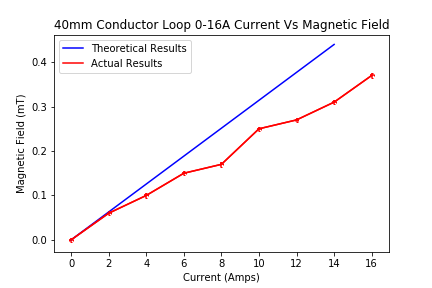
\includegraphics[scale=0.9]{Images/Conductors/40mm_Conductor_Loop_0-16A_Graph.png}
\caption{40mm Conductor Loop 0-16A Current Vs Magnetic Field}
\label{40mm CL Current Vs Magnetic Field Graph}
\end{figure}
\begin{table}[H]
\begin{center}
 \begin{tabular}{|c||c|c|c|c|c|c|c|c|c|}
 \hline
 \multicolumn{10}{|c|}{Actual Results} \\
 \hline
 Current (Amps) & 0 & 2 & 4 & 6 & 8 & 10 & 12 & 14 & 16 \\
 \hline
 Magnetic Field (mT) & 0.00 & 0.06 & 0.10 & 0.15 & 0.17 & 0.25 & 0.27 & 0.31 & 0.37 \\
 \hline
 \hline
 \multicolumn{10}{|c|}{Theoretical Results} \\
 \hline
 Current (Amps) & 0 & 2 & 4 & 6 & 8 & 10 & 12 & 14 & 16 \\
 \hline
 Magnetic Field (mT) & 0.00 & 0.06 & 0.13 & 0.19 & 0.25 & 0.31 & 0.38 & 0.44 & 0.50 \\
 \hline
 \end{tabular}
 \caption{40mm Conductor Loop 0-16A Current vs Magnetic Field}
 \label{40mm CL Current Vs Magnetic Field Table}
\end{center}
\end{table}

Utilizing the 40mm diameter conductor loop, a direct correlation between current and the magnetic field can be shown, it was theoretically deduced that as the current was increased using \cref{Conductor Loop Eq}, so would the magnetic field \cref{40mm CL Current Vs Magnetic Field Graph}. In a physical simulation by keeping the axial B-probe stationary and only manipulating the current, it shows that the magnetic field will increase also, thus proving the theoretical anticipation. Thus proving that current directly affects the magnetic field of a conductor loop. \\

Within \cref{40mm CL Current Vs Magnetic Field Graph}, it shows a slight deviation of the actual data to that of the theory, though not within the error bars thus being outside the approved error analysis \cref{Error Analysis}. As the conductor loop or the axial B-probe was moved, external factors \cref{Error Analysis} must take the blame for the error. 

\begin{figure}[H]
\centering
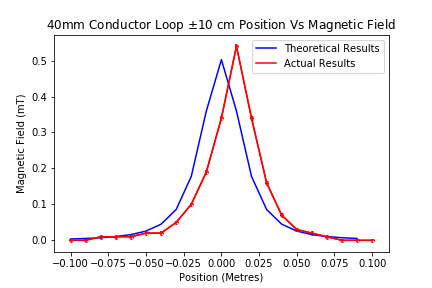
\includegraphics[scale=0.7]{Images/Conductors/40mm_CL_Position(cm)_Vs_Magnetic_Field_Graph.png}
\caption{40mm Conductor Loop $\pm10$cm Position vs Magnetic Field}
\label{40mm CL Positon Vs Magnetic Field Graph}
\end{figure}

\begin{table}[H]
\begin{center}
 \footnotesize
 \begin{tabular}{|c||c|c|c|c|c|c|c|c|c|c|c|}
 \hline
 \multicolumn{12}{|c|}{Actual Results} \\
 \hline
 Position (cm) & 0 & +1 & +2 & +3 & +4 & +5 & +6 & +7 & +8 & +9 & +10 \\
 \hline
 Magnetic Field (mT) & 0.34 & 0.54 & 0.34 & 0.16 & 0.07 & 0.03 & 0.02 & 0.01 & 0.00 & 0.00 & 0.00 \\
 \hline \hline
 Position (cm) & 0 & -1 & -2 & -3 & -4 & -5 & -6 & -7 & -8 & -9 & -10 \\
 \hline
 Magnetic Field (mT) & 0.34 & 0.19 & 0.10 & 0.05 & 0.02 & 0.02 & 0.01 & 0.01 & 0.01 & 0.00 & 0.00 \\
 \hline
 \hline
 \multicolumn{12}{|c|}{Theoretical Results} \\
 \hline
  Position (cm) & 0 & +1 & +2 & +3 & +4 & +5 & +6 & +7 & +8 & +9 & +10 \\
 \hline
 Magnetic Field (mT) & 0.50 & 0.35 & 0.17 & 0.08 & 0.04 & 0.02 & 0.01 & 0.01 & 0.00 & 0.00 & 0.00 \\
 \hline \hline
 Position (cm) & 0 & -1 & -2 & -3 & -4 & -5 & -6 & -7 & -8 & -9 & -10 \\
 \hline
 Magnetic Field (mT) & 0.50 & 0.35 & 0.17 & 0.08 & 0.04 & 0.02 & 0.01 & 0.01 & 0.00 & 0.00 & 0.00 \\
 \hline
 \end{tabular}
 \caption{40mm Conductor Loop $\pm10$cm Position vs Magnetic Field}
 \label{40mm CL Postion Vs Magnetic Field Table}
\end{center}
\end{table}

\begin{figure}[H]
\centering
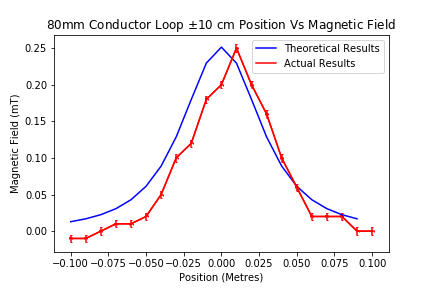
\includegraphics[scale=0.7]{Images/Conductors/80mm_CL_Position(cm)_Vs_Magnetic_Field_Graph.png}
\caption{80mm Conductor Loop $\pm10$cm Position vs Magnetic Field}
\label{80mm CL Positon Vs Magnetic Field Graph}
\end{figure}

\begin{table}[H]
\begin{center}
 \footnotesize
 \begin{tabular}{|c||c|c|c|c|c|c|c|c|c|c|c|}
 \hline
 \multicolumn{12}{|c|}{Actual Results} \\
 \hline
 Position (cm) & 0 & +1 & +2 & +3 & +4 & +5 & +6 & +7 & +8 & +9 & +10 \\
 \hline
 Magnetic Field (mT) & 0.20 & 0.25 & 0.20 & 0.15 & 0.10 & 0.06 & 0.02 & 0.02 & 0.02 & 0.00 & 0.00 \\
 \hline
 Position (cm) & 0 & -1 & -2 & -3 & -4 & -5 & -6 & -7 & -8 & -9 & -10 \\
 \hline
 Magnetic Field (mT) & 0.20 & 0.18 & 0.12 & 0.10 & 0.05 & 0.02 & 0.01 & 0.01 & 0.00 & -0.01 & -0.01 \\
 \hline
 \hline
 \multicolumn{12}{|c|}{Theoretical Results} \\
 \hline
 Position (cm) & 0 & +1 & +2 & +3 & +4 & +5 & +6 & +7 & +8 & +9 & +10 \\
 \hline
 Magnetic Field (mT) & 0.25 & 0.22 & 0.17 & 0.12 & 0.08 & 0.06 & 0.04 & 0.03 & 0.02 & 0.01 & 0.01 \\
 \hline
 Position (cm) & 0 & -1 & -2 & -3 & -4 & -5 & -6 & -7 & -8 & -9 & -10 \\
 \hline
 Magnetic Field (mT) & 0.25 & 0.22 & 0.17 & 0.12 & 0.08 & 0.06 & 0.04 & 0.03 & 0.02 & 0.01 & 0.01 \\
 \hline
 \end{tabular}
 \caption{80mm Conductor Loop $\pm10$cm Position vs Magnetic Field}
 \label{80mm CL Postion Vs Magnetic Field Table}
\end{center}
\end{table}

\begin{figure}[H]
\centering
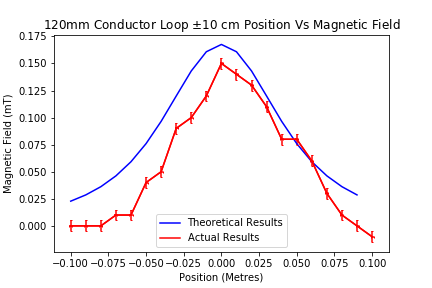
\includegraphics[scale=0.7]{Images/Conductors/120mm_CL_Position(cm)_Vs_Magnetic_Field_Graph.png}
\caption{120mm Conductor Loop $\pm10$cm Position vs Magnetic Field}
\label{120mm CL Positon Vs Magnetic Field Graph}
\end{figure}

\begin{table}[H]
\begin{center}
 \footnotesize
 \begin{tabular}{|c||c|c|c|c|c|c|c|c|c|c|c|}
 \hline
 \multicolumn{12}{|c|}{Actual Results} \\
 \hline
 Position (cm) & 0 & +1 & +2 & +3 & +4 & +5 & +6 & +7 & +8 & +9 & +10 \\
 \hline
 Magnetic Field (mT) & 0.15 & 0.14 & 0.13 & 0.11 & 0.08 & 0.08 & 0.06 & 0.03 & 0.01 & 0.00 & -0.01 \\
 \hline \hline
 Position (cm) & 0 & -1 & -2 & -3 & -4 & -5 & -6 & -7 & -8 & -9 & -10 \\
 \hline
 Magnetic Field (mT) & 0.15 & 0.12 & 0.10 & 0.19 & 0.05 & 0.04 & 0.01 & 0.01 & 0.00 & 0.00 & 0.00 \\
 \hline
 \hline
 \multicolumn{12}{|c|}{Theoretical Results} \\
 \hline
 Position (cm) & 0 & +1 & +2 & +3 & +4 & +5 & +6 & +7 & +8 & +9 & +10 \\
 \hline
 Magnetic Field (mT) & 0.17 & 0.16 & 0.14 & 0.11 & 0.09 & 0.07 & 0.05 & 0.04 & 0.03 & 0.02 & 0.02 \\
 \hline \hline
 Position (cm) & 0 & -1 & -2 & -3 & -4 & -5 & -6 & -7 & -8 & -9 & -10 \\
 \hline
 Magnetic Field (mT) & 0.17 & 0.16 & 0.14 & 0.11 & 0.09 & 0.07 & 0.05 & 0.04 & 0.03 & 0.02 & 0.02 \\
 \hline
 \end{tabular}
 \caption{120mm Conductor Loop $\pm10$cm Position vs Magnetic Field}
 \label{120mm CL Postion Vs Magnetic Field Table}
\end{center}
\end{table}

Though proving a correlation between current and the magnetic field, molding a new relationship between distance and the magnetic field is also imperative to understanding how magnetic fields are affected. Much like \cref{40mm CL Current Vs Magnetic Field Graph} a strong relationship is proved with the theory as \cref{40mm CL Positon Vs Magnetic Field Graph}, \cref{80mm CL Positon Vs Magnetic Field Graph} and \cref{120mm CL Positon Vs Magnetic Field Graph} gives insight on the shape of the magnetic field of this conductor loop. Where the magnetic field branches outwards and becomes larger and less strong. \\

As the conductor loop was moved instead of the axial B-probe, thus utilizing a 0.005m error, but as the conductor is too be tightened back onto the track, a possible error arises where the axial B-probe is not centred thus giving inaccurate readings when compared with the theoretical results. The theoretical results proven by \cref{Conductor Loop Eq} indicates gradual curves as it peaks at zero where the centre of the magnetic field.

%---------------------------------------------------------------------------
\subsubsection{Conductor loop comparison}

\begin{figure}[H]
\centering
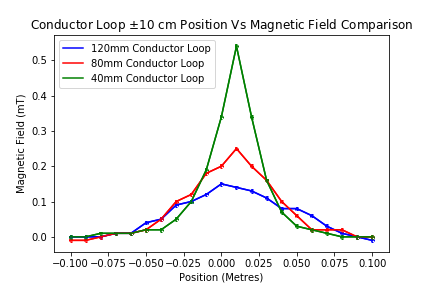
\includegraphics[scale=0.9]{Images/Conductors/Conductor_Loop_Comparsion_Graph.png}
\caption{Conductors Position vs Magnetic Field}
\label{Conductors Positon Vs Magnetic Field Graph}
\end{figure}

By comparing the actual results obtained in this experiment (\cref{Conductors Positon Vs Magnetic Field Graph}), a pattern emerges that suggests that the smaller the conductor loop produced a smaller denser magnetic field. The magnetic field of a 120mm conductor loop is much bigger than that of the 40mm conductor loop but with such large changes of the axial direction in comparison of the size of the 120mm conductor loop, gives weaker values as it's quickly expands further in diameter than the 40mm conductor loop and less in width/length.

%---------------------------------------------------------------------------
\subsubsection{Straight conductor}

\begin{figure}[H]
\centering
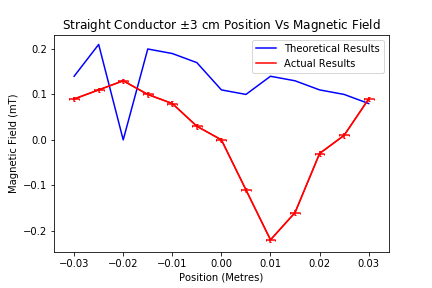
\includegraphics[scale=0.7]{Images/Conductors/Straight_Conductor_Position_Vs_Magnetic_Field.png}
\caption{Straight Conductor $\pm3$cm Position vs Magnetic Field}
\label{Straight Conductor Positon Vs Magnetic Field Graph}
\end{figure}

\begin{table}[H]
\begin{center}
 \begin{tabular}{|c||c|c|c|c|c|c|c|c|c|c|c|}
 \hline
  \multicolumn{8}{|c|}{Actual Results} \\
 \hline
 Position (cm) & 0 & +0.5 & +1.0 & +1.5 & +2.0 & +2.5 & +3.0 \\
 \hline
 Magnetic Field (mT) & 0.00 & -0.11 & -0.22 & -0.16 & -0.03 & 0.01 & 0.09 \\
 \hline \hline
 Position (cm) & 0 & -0.5 & -1.0 & -1.5 & -2.0 & -2.5 & -3.0 \\
 \hline
 Magnetic Field (mT) & 0.00 & 0.03 & 0.08 & 0.10 & 0.13 & 0.11 & 0.09 \\
 \hline
 \hline
 \multicolumn{8}{|c|}{Theoretical Results} \\
 \hline
  Position (cm) & 0 & +0.5 & +1.0 & +1.5 & +2.0 & +2.5 & +3.0 \\
 \hline
 Magnetic Field (mT) & 0.11 & 0.10 & 0.14 & 0.13 & 0.11 & 0.10 & 0.08 \\
 \hline \hline
 Position (cm) & 0 & -0.5 & -1.0 & -1.5 & -2.0 & -2.5 & -3.0 \\
 \hline
 Magnetic Field (mT) & 0.11 & 0.17 & 0.19 & 0.20 & 0.00 & 0.21 & 0.14 \\
 \hline
 \end{tabular}
 \caption{Straight Conductor $\pm3$cm Position vs Magnetic Field}
 \label{Straight Conductor Postion Vs Magnetic Field Table}
\end{center}
\end{table}

The straight conductor is by far the trickiest of all the conductors this experiment covers, to begin at an offset and then consider said offset while moving the axial B-probe along the length of the conductor causing a error in itself and the measuring device is being moved and out of alignment. The axial B-probe has also been placed in the wrong direction measuring in the wrong polarity.

%---------------------------------------------------------------------------
\subsection{Axial magnetic field of an air solenoid}
\label{air section}

\begin{figure}[H]
\centering
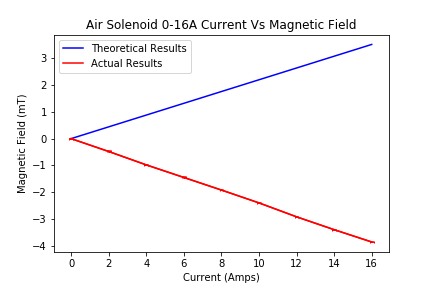
\includegraphics[scale=0.7]{Images/Air_Solenoid/Air_Solenoid_0-16A_Graph.png}
\caption{Air Solenoid 0-16A Current Vs Magnetic Field}
\label{Air Solenoid Current Vs Magnetic Field Graph}
\end{figure}

\begin{table}[H]
\begin{center}
 \begin{tabular}{|c||c|c|c|c|c|c|c|c|c|}
  \hline
  \multicolumn{10}{|c|}{Actual Results} \\
  \hline
  Current (Amps) & 0 & 2 & 4 & 6 & 8 & 10 & 12 & 14 & 16 \\
  \hline
  Magnetic Field (mT) & 0.00 & -0.48 & -0.98 & -1.45 & -1.92 & -2.40 & -2.92 & -3.40 & -3.86 \\
  \hline
  \hline
  \multicolumn{10}{|c|}{Theoretical Results} \\
  \hline
  Current (Amps) & 0 & 2 & 4 & 6 & 8 & 10 & 12 & 14 & 16 \\
  \hline
  Magnetic Field (mT) & 0.00 & 0.43 & 0.87 & 1.31 & 1.75 & 2.19 & 2.63 & 3.07 & 3.51 \\
 \hline
 \end{tabular}
 \caption{Air Solenoid 0-16A Current Vs Magnetic Field}
 \label{Air Solenoid Current Vs Magnetic Field Table}
\end{center}
\end{table}


\begin{figure}[H]
\centering
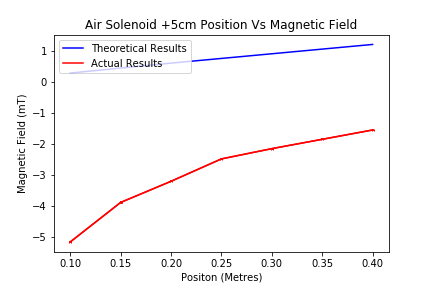
\includegraphics[scale=0.7]{Images/Air_Solenoid/Air_Solenoid_Position_Vs_Magnetic_Field.png}
\caption{Air Solenoid $\pm5$cm Position Vs Magnetic Field}
\label{Air Solenoid Position Vs Magnetic Field Graph}
\end{figure}

\begin{table}[H]
\begin{center}
 \begin{tabular}{|c||c|c|c|c|c|c|c|}
  \hline
  \multicolumn{8}{|c|}{Actual Results} \\
  \hline
  \hline
  Position (cm)  & 10 & 15 & 20 & 25 & 30 & 35 & 40 \\
  \hline
  Magnetic Field (mT) & -5.15 & -3.88 & -3.20 & -2.48 & -2.15 & -1.85 & -1.55 \\
  \hline
  \hline
  \multicolumn{8}{|c|}{Theoretical Results} \\
  \hline
  Position (cm)  & 10 & 15 & 20 & 25 & 30 & 35 & 40 \\
  \hline
  Magnetic Field (mT) & 0.28 & 0.44 & 0.60 & 0.75 & 0.90 & 1.05 & 1.20 \\
  \hline
 \end{tabular}
 \caption{Air Solenoid $\pm5$cm Position Vs Magnetic Field}
 \label{Air Solenoid 5 Position Vs Magnetic Field Table}
\end{center}
\end{table}

\begin{figure}[H]
\centering
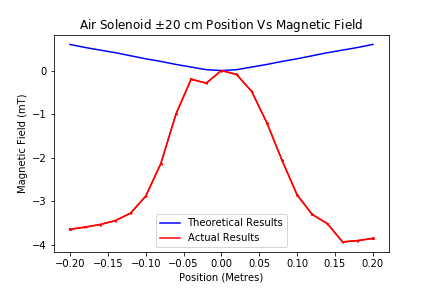
\includegraphics[scale=0.7]{Images/Air_Solenoid/Air_Solenoid_20_Position_Vs_Magnetic_Field.png}
 \caption{Air Solenoid $\pm2$cm Position Vs Magnetic Field}
 \label{Air Solenoid 20 Position Vs Magnetic Field graph}
\end{figure}

\begin{table}[H]
\begin{center}
 \footnotesize
 \begin{tabular}{|c||c|c|c|c|c|c|c|c|c|c|c|}
 \hline
 \multicolumn{12}{|c|}{Actual Results} \\
 \hline
 Position (cm) & 0 & +2 & +4 & +6 & +8 & +10 & +12 & +14 & +16 & +18 & +20 \\
 \hline
 Magnetic Field (mT) & 0.00 & -0.09 & -0.48 & -1.20 & -2.06 & -2.86 & -3.31 & -3.52 & -3.94 & -3.91 & -3.86 \\
 \hline \hline
 Position (cm) & 0 & -2 & -4 & -6 & -8 & -10 & -12 & -14 & -16 & -18 & -20 \\
 \hline
 Magnetic Field (mT) & 0.00 & -0.29 & -0.20 & -1.00 & -2.14 & -2.89 & -3.28 & -3.45 & -3.54 & -3.60 & -3.65 \\
 \hline
 \hline
 \multicolumn{12}{|c|}{Theoretical Results} \\
 \hline
 Position (cm) & 0 & +2 & +4 & +6 & +8 & +10 & +12 & +14 & +16 & +18 & +20 \\
 \hline
 Magnetic Field (mT) & 0.00 & 0.02 & 0.08 & 0.14 & 0.21 & 0.27 & 0.34 & 0.41 & 0.47 & 0.53 & 0.60 \\
 \hline \hline
 Position (cm) & 0 & -2 & -4 & -6 & -8 & -10 & -12 & -14 & -16 & -18 & -20 \\
 \hline
 Magnetic Field (mT) & 0.00 & 0.02 & 0.08 & 0.14 & 0.21 & 0.27 & 0.34 & 0.41 & 0.47 & 0.53 & 0.60 \\
 \hline
 \end{tabular}
 \caption{Air Solenoid $\pm20$cm Position vs Magnetic Field}
 \label{Air Solenoid 20 Postion Vs Magnetic Field Table}
\end{center}
\end{table}

The polarity of the axial B-probe was inverted for \cref{Air Solenoid Current Vs Magnetic Field Graph} as if it was inverted the simulation would perfectly mimic the theoretical data, thus proving again a direct relationship between current and a conductor, in this case the air solenoid. Looking at another relationship; the distance and magnetic field of an air solenoid, \cref{Air Solenoid 5 Position Vs Magnetic Field Table} shows this, thus the axial B-probe was not zeroed and gave inaccurate values of the magnetic field, but in regards to the pattern of of the physical data compared to the theory, it shows a positive correlation. The analysis of \cref{Air Solenoid 20 Position Vs Magnetic Field graph} proves again the error of inaccurate data off a non zeroed axial B-probe, its also plausible that the polarity of the probe was inverted as the physical data shows a negative pattern compared to its theoretical relative. \\

The data given gives insight on the shape of the magnetic field as it flows through the air solenoid and extrudes outwards at the solenoid and circles round, it can most likely be said that increasing the size of the magnetic field is done by increasing the current flowing through the solenoid and elongating the length of the magnetic field is done by manipulating the air solenoids length.

%---------------------------------------------------------------------------
\subsection{Radial and tangential magnetic field of an Helmholtz coil}
\label{radial coil}

\begin{figure}[H]
\centering
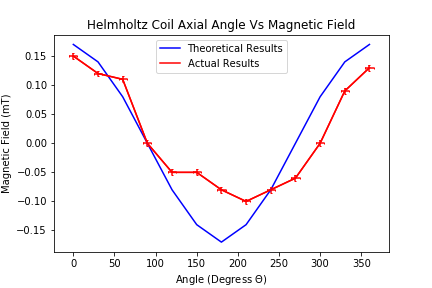
\includegraphics[scale=0.7]{Images/Helmholtz_Coils/Helmholtz_Coil_Angle_1_Vs_Magnetic_Field.png}
\caption{Helmholtz Coil Axial Angle vs Magnetic Field}
\label{Helmholtz Coil Axial Angle Vs Magnetic Field Graph}
\end{figure}

\begin{table}[H]
\begin{center}
 \begin{tabular}{|c||c|c|c|c|c|c|c|c|c|c|c|c|c|}
 \hline
 \multicolumn{8}{|c|}{Actual Results} \\
 \hline
 Angle ($\theta$) & 0 & 30 & 60 & 90 & 120 & 150 & 180 \\
 \hline
 Magnetic Field (mT) & 0.15 & 0.12 & 0.11 & 0.00 & -0.05 & -0.05 & -0.08 \\
 \hline \hline
 Angle ($\theta$) &  & 210 & 240 & 270 & 300 & 330 & 360 \\
 \hline
 Magnetic Field (mT) & & -0.10 & -0.08 & -0.06 & 0.00 & 0.09 & 0.13 \\
 \hline
 \hline
 \multicolumn{8}{|c|}{Theoretical Results} \\
 \hline
 Angle ($\theta$) & 0 & 30 & 60 & 90 & 120 & 150 & 180 \\
 \hline
 Magnetic Field (mT) & 0.17 & 0.14 & 0.08 & 0.00 & -0.08 & -0.14 & -0.17 \\
 \hline \hline
 Angle ($\theta$) &  & 210 & 240 & 270 & 300 & 330 & 360 \\
 \hline
 Magnetic Field (mT) & & -0.08 & -0.06 & 0.00 & 0.09 & 0.13 & 0.15 \\
 \hline
 \end{tabular}
 \caption{Helmholtz Coil Axial Angle vs Magnetic Field}
 \label{Helmholtz Coil Axial Angle Vs Magnetic Field Table}
\end{center}
\end{table}

\begin{figure}[H]
\centering
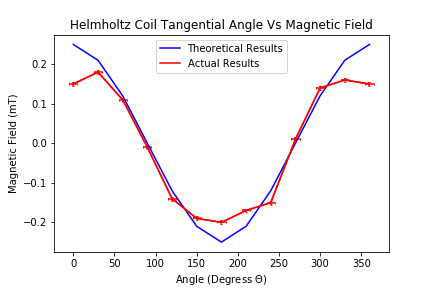
\includegraphics[scale=0.7]{Images/Helmholtz_Coils/Helmholtz_Coil_Angle_2_Vs_Magnetic_Field.png}
\caption{Helmholtz Coil Tangential Angle vs Magnetic Field}
\label{Helmholtz Coil Tangential Angle Vs Magnetic Field Graph}
\end{figure}

\begin{table}[H]
\begin{center}
 \begin{tabular}{|c||c|c|c|c|c|c|c|c|c|c|c|c|c|}
 \hline
 \multicolumn{8}{|c|}{Actual Results} \\
 \hline
 Angle ($\theta$) & 0 & 30 & 60 & 90 & 120 & 150 & 180 \\
 \hline
 Magnetic Field (mT) & 0.15 & 0.18 & 0.11 & -0.01 & -0.14 & -0.19 & -0.20 \\
 \hline \hline
 Angle ($\theta$) &  & 210 & 240 & 270 & 300 & 330 & 360 \\
 \hline
 Magnetic Field (mT) & & -0.17 & -0.15 & 0.01 & 0.14 & 0.16 & 0.15 \\
 \hline
 \hline
 \multicolumn{8}{|c|}{Theoretical Results} \\
 \hline
 Angle ($\theta$) & 0 & 30 & 60 & 90 & 120 & 150 & 180 \\
 \hline
 Magnetic Field (mT) & 0.25 & 0.21 & 0.12 & 0.00 & -0.12 & -0.21 & -0.25 \\
 \hline \hline
 Angle ($\theta$) &  & 210 & 240 & 270 & 300 & 330 & 360 \\
 \hline
 Magnetic Field (mT) & & -0.21 & -0.12 & 0.0 & 0.12 & 0.21 & 0.25 \\
 \hline
 \end{tabular}
 \caption{Helmholtz Coil Tangential Angle vs Magnetic Field}
 \label{Helmholtz Coil Tangential Angle Vs Magnetic Field Table}
\end{center}
\end{table}

Great care is taken to ensure that this apparatus setup is correct to obtained the desired values for the magnetic field, this set up focused on the relationship of the radial and tangential angle of the coil and the effect of the magnetic field. Though the physical simulation matched the theoretical data it shows the shape of the magnetic field, it shows that the field flows through the coil itself and extrudes at one end and circles round the exterior of the coil to flow back into the centre of the coil again. This is confirmed when the coil hit 90\textdegree, 270\textdegree, thus no field is being emitted.\\

This set up shows not only the size as the other setups have shown but the shape in which the magnetic field operates, how the magnetic field operates in a full 360\textdegree's. This is not clearly shown as the axial B-probe is fixed thus provided the results with null values but it can imaged as the graphs shows the magnetic fields shape being unchanged.

%---------------------------------------------------------------------------
\subsection{Axial magnetic field of a pair Helmholtz coil}
\label{Axial magnetic field of a pair Helmholtz coil}

\begin{figure}[H]
\centering
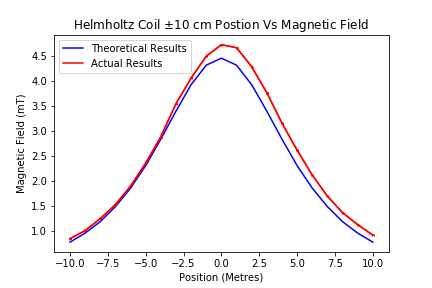
\includegraphics[scale=0.7]{Images/Helmholtz_Coils/Helmholtz_Coil_Position_Vs_Magnetic_Field.png}
\caption{Helmholtz Coils $\pm10$cm Position vs Magnetic Field}
\label{Helmholtz Coil 10 Positon Vs Magnetic Field Graph}
\end{figure}

\begin{table}[H]
\begin{center}
 \footnotesize
 \begin{tabular}{|c||c|c|c|c|c|c|c|c|c|c|c|}
 \hline
 \multicolumn{12}{|c|}{Actual Results} \\
 \hline
 Position (cm) & 0 & +1 & +2 & +3 & +4 & +5 & +6 & +7 & +8 & +9 & +10 \\
 \hline
 Magnetic Field (mT) & 4.73 & 4.67 & 4.29 & 3.77 & 3.16 & 2.62 & 2.12 & 1.70 & 1.37 & 1.13 & 0.92 \\
 \hline \hline
 Position (cm) & 0 & -1 & -2 & -3 & -4 & -5 & -6 & -7 & -8 & -9 & -10 \\
 \hline
 Magnetic Field (mT) & 4.73 & 4.50 & 4.06 & 3.55 & 2.89 & 2.36 & 1.90 & 1.53 & 1.25 & 1.01 & 0.85 \\
 \hline
 \hline
 \multicolumn{12}{|c|}{Theoretical Results} \\
 \hline
 Position (cm) & 0 & +1 & +2 & +3 & +4 & +5 & +6 & +7 & +8 & +9 & +10 \\
 \hline
 Magnetic Field (mT) & 4.46 & 4.32 & 3.93 & 3.40 & 2.84 & 2.31 & 1.86 & 1.49 & 1.19 & 0.96 & 0.78 \\
 \hline \hline
 Position (cm) & 0 & -1 & -2 & -3 & -4 & -5 & -6 & -7 & -8 & -9 & -10 \\
 \hline
 Magnetic Field (mT) & 4.46 & 4.32 & 3.93 & 3.40 & 2.84 & 2.31 & 1.86 & 1.49 & 1.19 & 0.96 & 0.78 \\
 \hline
 \end{tabular}
 \caption{Helmholtz Coils $\pm10$cm Position vs Magnetic Field}
 \label{Helmholtz Coil Postion Vs Magnetic Field Table}
\end{center}
\end{table}

\begin{figure}[H]
\centering
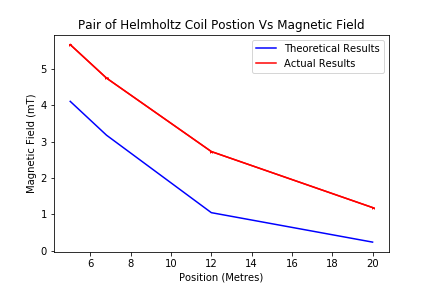
\includegraphics[scale=0.7]{Images/Helmholtz_Coils/Pair_Helmholtz_Coil_Position_Vs_Magnetic_Field.png}
\caption{Pair of Helmholtz Coils Position Vs Magnetic Field}
\label{Pair of Helmholtz Coils Position Vs Magnetic Field Graph}
\end{figure}

\begin{table}[H]
\begin{center}
 \begin{tabular}{|c||c|c|c|c|c|c|c|}
 \hline
 \multicolumn{5}{|c|}{Actual Results} \\
 \hline
 Position (cm) & 5.0 & 6.8 & 12.0 & 20.0 \\
 \hline
 Magnetic Field (mT) & 5.67 & 4.75 & 2.73 & 1.19 \\
 \hline
 \hline
 \multicolumn{5}{|c|}{Theoretical Results} \\
 \hline
 Position (cm) & 5.0 & 6.8 & 12.0 & 20.0 \\
 \hline
 Magnetic Field (mT) & 4.11 & 3.18 & 1.05 & 0.24 \\
 \hline
 \end{tabular}
 \caption{Pair of Helmholtz Coils Position Vs Magnetic Field}
 \label{Pair of Helmholtz Coils Position Vs Magnetic Field Table}
\end{center}
\end{table}

Confirming the analysis of \cref{radial coil} about the shape the Helmholtz coil produces, its shape quite clear in \cref{Helmholtz Coil 10 Positon Vs Magnetic Field Graph} as it completes a full rotation of each half of the coil. The relationship between the angle and magnetic field are not only confirmed but also provide insight on the confirmation of the shape of the magnetic field in coils. \\

The second part to this stage of the physical simulation improves the insight given above, by using two Helmholtz coils instead of one shows us the principle of superposition come into effect. The two coils are set so they their magnetic fields combine and thus in the middle of both coils, the principle of superposition lies at the weakest values of the magnetic field. This set up provides insight that the magnetic fields of two separate coils can combine, and if posed opposite polarities, this is explained further later on \cref{questions}.

\subsection{Questions}
\label{questions}

"What is the direction and strength of the Earth's magnetic field in the physics laboratory?" \cite{Exp.5-2019}\\

To answer this question from this experiment alone, the magnetic field of the whole experiment favours north-western direction which corresponds with a shape that Earths magnetic field make, this shape is mimicked in \cref{loop seciton} and \cref{air section} as due to Earths poles. The poles act much like the air solenoid and bursts out canvasing the entire spherical shape of the Earth much like the conductor loops.  \\

"If the pair of Helmholtz coils were wired in the other direct (one clockwise, the other anti-clockwise), what would the magnetic field be like between the Helmholtz coils?"\cite{Exp.5-2019}\\

Within \cref{Axial magnetic field of a pair Helmholtz coil} the experiment looked at this question, even though the experiment was set up so both Helmholtz coils were either clockwise or anti-clockwise so the current flowing through both of the coils are flowing in the same direction. The experiment saw the principle of superposition take effect in between both of the coils, where the magnetic field was at its weakest, this shows where the two separate magnetic field overlap and merge. If faced opposite each other with the current moving in the anti of each other then the magnetic fields would clash and a cancel thus leaving an area where the magnetic field jumps from positive to negative. In short the two individual magnetic field would never combine and thus resist each other. 

%---------------------------------------------------------------------------
%	DISCUSSION
%---------------------------------------------------------------------------
\section{Discussion}
\label{diss}

This experiment covered a lot of ground regarding how multiple scenarios affect the how the magnetic field behaves, but in this practical simulation it can been seen that compared to theoretical result, multiple errors were made. Whether it be Human error or equipment error, this physical simulation still gave insight in how magnetic field at affected and how they are formed under different conductors, also how they change shape given certain external factors. \\

Furthermore it can be said that not only this experiment but this physical simulation proves that the magnetic field can be deduced by theoretical methods but alas the theory is flawed under the influence of environmental factors, the physical simulation was conducted in a laboratory full of computers, phones and many more, most importantly the laboratory is surrounded by electrical cabling carrying current constantly, it can also be stated that the Earths own magnetic field altered the results of this physical simulation. \\

%---------------------------------------------------------------------------
%	CONCLUSION
%---------------------------------------------------------------------------
\section{Conclusion}

As stated in \cref{diss}, there is a direct relationship between the magnetic field produced by current, different sizes and shapes of conductors, distance and angle. This is proven throughout this physical simulation, under the extreme external factors altering this simulation, it can be stated that the theory even though mathematically accurate cannot fully relate to a physical simulation. \\

This physical simulation proved exactly what the theory suggested, change under duress. By changing multiple factors the physical results still showed change like the theory suggested, these physical multiple changes not only effected the strength of the magnetic field but its shape and size.

%---------------------------------------------------------------------------
%	REFERENCES
%---------------------------------------------------------------------------
%\end{multicols}
\bibliographystyle{plain}
\bibliography{mybib.bib}
\end{document}